\subsubsection{Implementacion 1}

\textbf{Explicación assembler}

En esta implementación modificamos de a un pixel a la vez, comenzando a recorrer la primer fila de la matriz que representa a la imagen hasta que ésta se acabe y luego repetir el proceso con la fila siguiente hasta alcanzar el borde cuyos píxeles no son modificados. Para calcular los valores resultantes de cada componente del pixel, mantenemos en cada iteración un puntero al primero de los 9 píxeles necesarios para el cálculo correspondiente al filtro Blur (ver enunciado).

Para poder calcular correctamente los píxeles, debemos tener cuidado de no utilizar el valor modificado de los píxeles vecinos que utilizamos para realizar las cuentas.

Para lograr lo dicho anteriormente, al comienzo del código creamos un vector del tamaño equivalente a una fila de la imagen, que lo vamos a utilizar para guardar temporalmente n píxeles, siendo n la cantidad de píxeles que tiene una fila.

Este vector lo inicializamos con los píxeles de la primera fila de la imagen. Aunque ésto no es necesario, de esta manera nos evitamos realizar el caso base correspondiente a la primera fila de la imagen, ya que ésta no se modifica, fuera del ciclo correspondiente.

Nuestra función opera de la siguiente manera:
Hay dos ciclos, uno dentro del otro, en donde el ciclo externo itera sobre las filas y el ciclo interno lo hace sobre las columnas.

\begin{figure}[ht!]
\centering
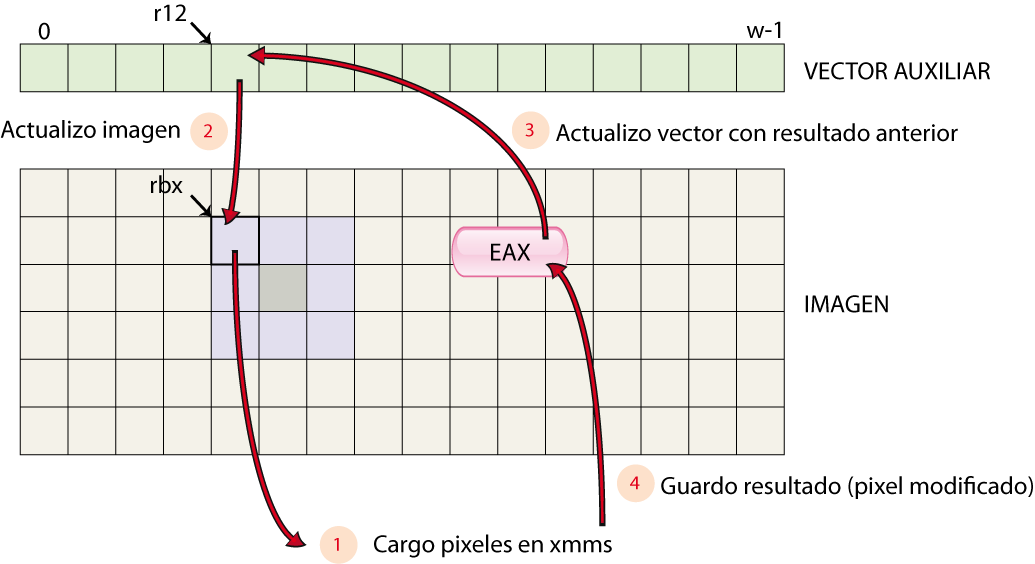
\includegraphics[width=120mm]{imagenes/blur/blur1-figura1.png}
\caption{Desarrollo de Blur-ASM1.}
\end{figure}

1) En el ciclo interno guardamos en 3 registros xmm, en nuestro caso xmm0, xmm2 y xmm4, los primeros cuatro píxeles consecutivos de 3 filas contiguas. De estos 4 píxeles vamos a necesitar solamente 3, de forma que los píxeles que utilicemos sean los píxeles vecinos al pixel que vamos a modificar y a si mismo.

\begin{figure}[ht!]
\centering
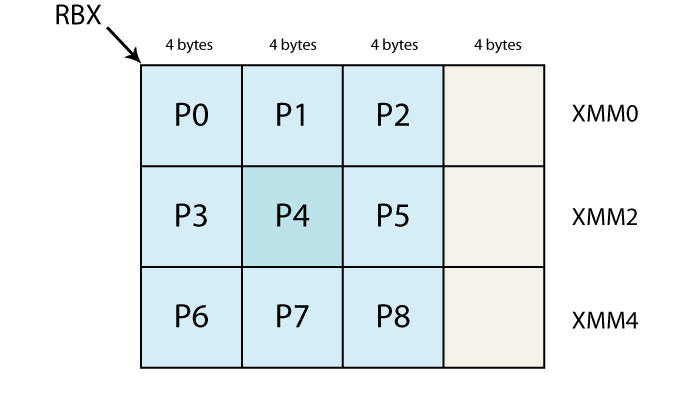
\includegraphics[width=70mm]{imagenes/blur/blur1-figura2.png}
\caption{Desarrollo de Blur-ASM1.}
\end{figure}

2) Una vez que los píxeles de la imagen están en los registros, modificamos el pixel de la imagen ubicado en la menor posición intercambiándolo con el pixel correspondiente del vector creado previamente, que contiene el pixel ya modificado correspondiente a esa posición de memoria.

3) Ahora que ya utilizamos la posición del vector para actualizar la imagen, guardamos el resultado que habíamos obtenido en la iteración anterior (que guardamos en EAX) en el vector. En caso que sea el primer pixel de la fila, antes de entrar al ciclo de la nueva fila se guarda en EAX el pixel correspondiente.

4) Realizamos las operaciones necesarias con los datos y guardamos el resultado (el pixel modificado) en EAX.
Para sumar las componentes de los píxeles sin que ocurra overflow en nuestra representación, duplicamos el tamaño de cada una de ellas expandiendolas de byte a word. Dejamos dos píxeles en el registro en el que estaban (con el tamaño modificado) y los otros dos en otro registro xmm. 
Luego realizamos suma de words entre los registros, el resultado lo guardamos en xmm0. 
El siguiente paso es  shiftear a la derecha los registros xmm0, xmm2 y xmm4 y los sumamos para asi obtener en la parte baja del registro xmm0 la suma de los 9 pixeles involucrados.
Duplicamos el tamaño de cada componente a 32 bits para convertir a float y dividir por nueve cada uno de ellos. Una vez concluído ésto, volvemos a convertir las componentes a enteros, y volvemos a empaquetarlas a su tamaño original, de forma que quede el pixel resultante en la parte más baja del registro xmm0.
El resultado obtenido lo guardo en un registro para poder ubicarlo en el vector en la iteración siguiente. No lo podemos guardar en el vector ahora porque todavía necesitamos usar el valor correspondiente a esa posición en la próxima iteración.

\begin{figure}[ht!]
\centering
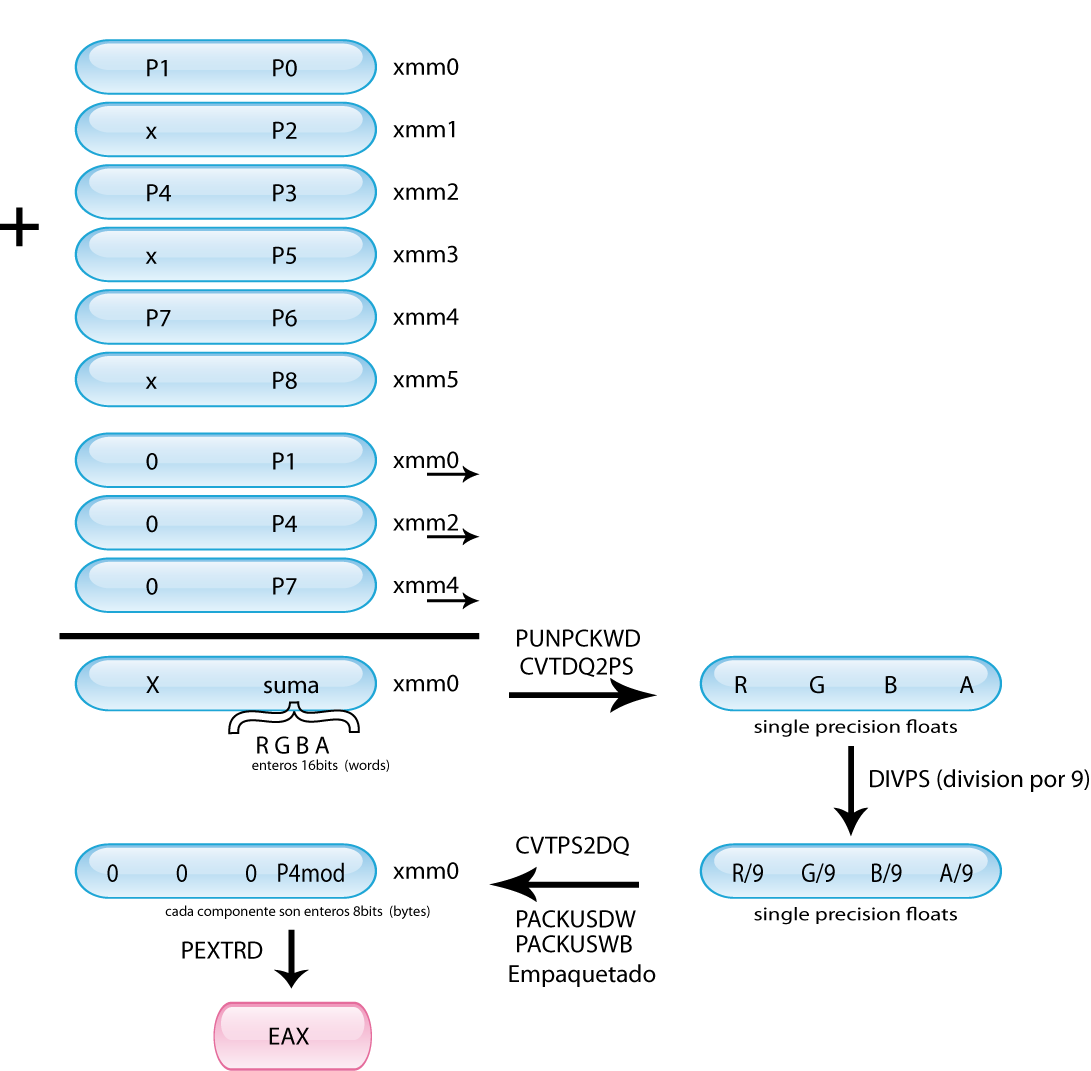
\includegraphics[width=100mm]{imagenes/blur/blur1-figura3.png}
\caption{Desarrollo de Blur-ASM1.}
\end{figure}

Caso Borde: Antes de volver a iterar en el ciclo externo, se realiza el caso borde del final de la fila, que es análogo a una iteración del ciclo interno. Cuando se llega a la última columna de pixeles que se debe modificar, retrocedemos con el puntero al pixel anterior y tomamos los ultimos 3 pixeles de cada registro en vez de los 3 primeros. (Si no hariamos ésto, en la ultima fila intentariamos acceder a memoria que no es nuestra).
Nota: Al finalizar el caso borde actualizamos el anteúltimo pixel de la fila y cargamos el resultado directo al vector, no hace falta guardarlo en EAX.

Una vez finalizado ésto, realizamos las operaciones necesarias para poder realizar la siguiente iteración del ciclo externo.

Al finalizar el ciclo de las filas, actualizamos la anteúltima fila con los valores modificados, guardados en el vector durante la última iteración del ciclo.


\subsubsection{Implementacion 2}

\textbf{Explicación assembler}

En esta implementación modificamos la imagen de a cuatro píxeles por vez, considerando a la imagen como una matriz de píxeles. El orden que seguimos para procesar los grupos de píxeles es: procesar los primeros cuatro píxeles de la imagen (sin contar los bordes) y hacer lo mismo con el siguiente grupo de píxeles hasta que llegamos al final de la fila, donde debemos procesar solo dos píxeles. Luego cambiamos de fila y repetimos el proceso hasta llegar a la última fila de la imagen.

Para lograr ésto debemos tener cuidado de no procesar píxeles con los valores modificados de sus vecinos. Al igual que en la anterior implementación, utilizamos un vector del tamaño de una fila de la matriz en donde guardaremos los valores modificados de la imagen hasta que hayamos utilizado a los píxeles que se deben reemplazar en todas las cuentas en las que se vean implicados.
Este vector es inicializado con los píxeles correspondientes a la primera fila de la imagen para evitar problemas en la primer iteración del ciclo cuando actualizamos la imagen.

\begin{figure}[ht!]
\centering
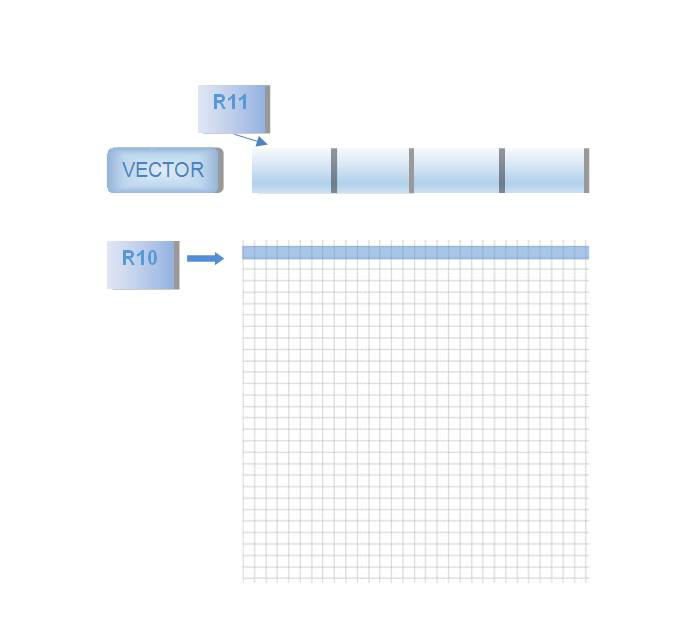
\includegraphics[width=90mm]{imagenes/blur/blur2-1.png}
\caption{Desarrollo de Blur-ASM2.}
\end{figure}

Luego de haber inicializado el vector, comenzamos con los ciclos para el procesamiento de los píxeles utilizando dos ciclos: un ciclo externo que recorre las filas y un ciclo interno que recorre las columnas, contenido por el primero.

Al comenzar el ciclo externo, inicializamos los registros para manipular los datos que se van a utilizar en el ciclo interno. Estos datos son el ancho de la fila, que es nuestra referencia a cantidad de iteraciones a realizar en el ciclo interno, un puntero a la dirección de memoria del primero de todos los píxeles que vamos a utilizar, y un puntero al inicio del vector.

Luego comienza a realizarse el ciclo interno.

Al comenzar el ciclo interno, utilizamos nueve registros xmm para guardar los grupos de cuatro píxeles de la siguiente forma:

\begin{figure}[ht!]
\centering
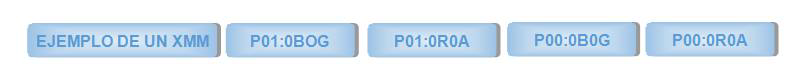
\includegraphics[width=120mm]{imagenes/blur/blur2-2.png}
\caption{Desarrollo de Blur-ASM2.}
\end{figure}

Una vez cargados los píxeles en los registros, procedemos a actualizar los cuatro píxeles de la imagen original con los cuatro píxeles correspondientes al vector creado. Es decir, actualizamos el valor de los píxeles que ya terminamos de utilizar, y de manera análoga a la implementación 1, cargamos en el vector el cuarto de los 4 pixeles que habíamos calculado en la iteración anterior y guardado en un registro, para no pisar los valores que necesitamos para actualizar la imagen.

Paso siguiente es duplicar el tamaño de las componentes de los píxeles en los registros xmm utilizados previamente. Como los registros ahora pasan a poder contener solamente dos píxeles, vamos a necesitar el doble de registros para poder guardar todos los píxeles necesarios.

\begin{figure}[ht!]
\centering
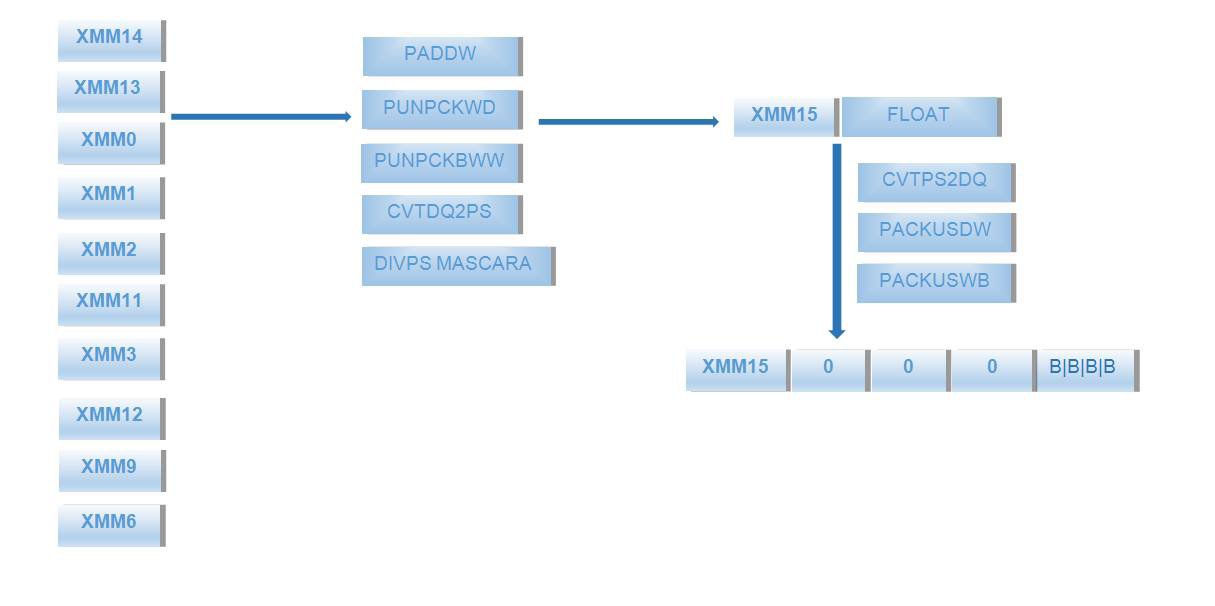
\includegraphics[width=120mm]{imagenes/blur/blur2-3.png}
\caption{Desarrollo de Blur-ASM2.}
\end{figure}

A continuación, realizamos las operaciones para calcular un pixel. Hacemos la sumatoria de las componentes de los píxeles, guardando el resultado en otro registro, transformamos ese resultado a punto flotante de precisión simple para poder divirlas a todas a la vez y obtener el promedio. Una vez calculado, lo transformamos nuevamente a entero.

Una vez calculado el pixel, lo transformo a su tamaño original, y copio el pixel al vector creado al comienzo del código. 

\begin{figure}[ht!]
\centering
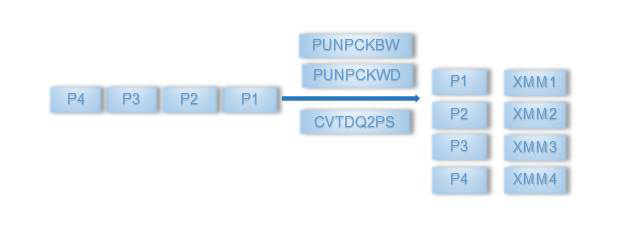
\includegraphics[width=100mm]{imagenes/blur/blur2-4.png}
\caption{Desarrollo de Blur-ASM2.}
\end{figure}

Para calcular los otros tres píxeles, el procedimiento es similar al recién descrito, teniendo en cuenta la ubicación de los píxeles necesarios en los registros utilizados. El cuarto pixel, como se menciona antes, se guarda provisoriamente en un registro pues el valor que le correspondería en el vector sera utilizado al comienzo del próximo ciclo.

Al finalizar el ciclo interno, debemos procesar los últimos dos píxeles de la fila iterada debido a que el ciclo sólo procesa de a cuatro píxeles. Este procesamiento es análogo a una iteración del ciclo interno, pero manipulando con precaución los registros debido a que usamos menor cantidad de píxeles y de cantidad de registros xmm.

Finalizado el procesamiento de estos dos píxeles, cambiamos la fila que vamos a iterar en el ciclo interno de la siguiente iteración del ciclo externo.

El ciclo externo termina cuando no hay más filas de la imagen que procesar, dejando las últimas dos filas de la imagen sin modificar, y las modificaciones de la anteúltima fila de la misma imagen en el vector creado por nosotros.

Cuando termina de realizarse el ciclo externo, debemos copiar los datos del vector a la anteúltima fila de la imagen, y con esto finaliza la función.